\documentclass[a4paper,12pt]{article}
\pagestyle{headings}
\usepackage[utf8]{inputenc}
\usepackage{aeguill} 
\usepackage{wrapfig}
\usepackage{graphicx}
\usepackage{gensymb}
\usepackage{fullpage}
\graphicspath{ {project_proposal_img/} }
 


\begin{document}

\begin{titlepage}
\begin{center}

% Upper part of the page. The '~' is needed because \\
% only works if a paragraph has started.
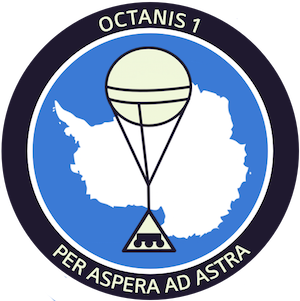
\includegraphics[width=0.35\textwidth]{patch}~\\[2cm]

\textsc{\Large Project Proposal}\\[0.5cm]

% Title
\huge \bfseries Octanis 1: A low-cost autonomous rover for Antarctica with real-time data transmission via satellite \\[0.4cm] 

\vspace{23pt}

\includegraphics[width=0.25\textwidth]{black_logo} \\
\vfill

% Bottom of the page
{\large \today} \\
\textsc{\small info@octanis.org | www.octanis.org}
\vspace{50pt}


\begin{table}[h!]
\centering
\vspace{1pt}
\begin{tabular}{ l  l  l }
	\textbf{Rev.} & \textbf{Changes} & \textbf{Authors} \\
	25.6.14 & Initial proposal & Sam Sulaimanov, Raffael Tschui, Ana Roldán, Pamela Canjura \\
	27.6.14 & Spanish version & Ana Roldán \\
	27.6.14 & German version & Raffael Tschui \\
\end{tabular}
\end{table}

\end{center}
\end{titlepage}

\tableofcontents

\pagebreak

\section{Introduction}
»octanis | discovery and exploration« \cite{octanis} is a student initiative to embark on ambitious and challenging projects together as multi-disciplinary students. Octanis 1 is our first mission to build a low-cost autonomous rover for polar, snow or ice covered regions. In this first iteration we will be specialising the rover for the coastal regions of Antarctica and its specific weather conditions. The rover will transmit sensor data like temperature, air pressure, relative humidity, current position and pose. There will be optical instruments on-board as well to sense obstacles and take pictures of the environment in its close vicinity. Other more specific environmental data collection is possible, but needs to be specially addressed due to the non-negligible power and weight requirements. These could be the concentration of an atmospheric gas, $\alpha, \beta, \gamma$ radiation levels or snow and ice sampling. \\ We have selected the periodic sampling of snow and ice to be the most suitable initial science mission for Octanis 1 \cite{krishnakant}. The rover will have a small hollow device capable of drilling into the surface ice or snow, melting the sample and analysing the pH.
\\ Energy will be provided by the solar panels on Octanis' surfaces and used throughout the Antarctic summer in combination with a battery pack. Communications will go through the Iridium satellite network \cite{iridium}, providing a low cost, low power and reliable data transmission at any location on Earth. 



\section{Mission Overview}

The aim of this mission, Octanis 1, is to provide a low-cost, low environmental impact rover platform for scientific experiments in cold to extremely cold environments. The rover will be small and light-weight enough to be carried on weather balloons. Its design will allow it to traverse icy terrain and be resistant to wind gusts. It will generate its own power with solar panels and regulate internal temperature as it's first priority. The rover will be on a four-wheel drive platform, each wheel being on a controllable strut, allowing it to drive in any orientation and right itself should it flip over. 


\subsection{Objectives}

\paragraph{Robotics}
A weather-proof, cold-resistant and light-weight rover shall be built that has a simple but solid hardware and software design. The rover must be able to complete a mission autonomously with assistance where necessary. A mission contains a movement path and sensing actions to be executed. Interrupting or aiding commands to be executed by the rover can be sent via the Internet to the rover. Energy generation and storage shall be dealt with in such a way that a mission can continue for several months without human interception.

\paragraph{Sensing}
The rover shall carry sensors on board to regularly record and transmit the state of the external and internal environment in a given location. It should provide a standard interface so that scientific instruments can be embedded and exchanged in a simple manner. All data transmitted to and from the rover shall be publicly available on the Internet in real-time. The rover shall have an interface to participate in a wider spread sensor network so that future rovers can work as a swarm.

\paragraph{Deployment}
Various methods of deploying the rover, long and short range, shall be evaluated and compared. Their costs and risks shall be weighed.


\paragraph{Open \& Reproducible} 
We are building Octanis based on the principles of the open source movement. All documentation, software and 3D models are available on our website for anyone to download, re-use and modify or even contribute. We use off-the-shelf parts where possible so that anyone with sufficient skills can build their own version of Octanis. We use fabrication techniques, like 3D printing, available to anyone having access to a workshop, fab lab \cite{fablab} or hackerspace \cite{hackerspace}. Access to these infrastructures is in many places available to everybody and at a low cost.
 

\subsection{Schedule}

Dates are for the year 2014 if not otherwise stated. The detailed dates for the science mission is to be determined in coordination with the collaborating Antarctic base. The project is managed transparently and in an agile manner and the development is strictly cyclic as to quickly incorporate urgent features as their need emerges. This method has worked well in the past and has proven to enable fast response to bugs and keep the costs low. Transparency is provided by opening all documentation to the public via GitHub \cite{octanisgithub} repositories. 

\begin{table}[h!]
\centering
\begin{tabular}{ l | l | l | c }

\bfseries{Code} & \bfseries{Mission Phase} & \bfseries{Dates} & \bfseries{Weeks} \\
\hline
A1 & Prototype Design \& Development & 1.6. - 1.10. & 12 \\
A2 & Software Development & 1.6. - 1.10. & 12 \\
B1 & Initial Testing & 1.10. - 14.10. & 2  \\
B2 & Drive \& Sampling Testing on Swiss Glacier & 14.10. - 14.11. & 4 \\
D & Mechanical Stress Testing & 14.11. - 21.12. & 1 \\
E & Energy Management Testing & 21.11. - 14.12. & 3 \\
F & Parachute Deployment Testing & 14.12. - 21.12. & 1 \\
0.1 & Deployment Opportunity in Antarctica & 14.2.2015 &  1 \\
0.2 & Deployment Opportunity in Antarctica & 1.12.2015 &  1 \\

\end{tabular}
\caption{Development timeline.}
\end{table}

After deployment, the schedule of the science mission will proceed as described in the following table. Note that during the whole mission there will be a constant satellite data connection to the rover. Basic heartbeat information and sensory data will be transmitted multiple times per day. Commands to intercept the mission progress can be sent at any time.

\begin{table}[h!]
\centering
\begin{tabular}{ l | l | c }
\bfseries{Code} & \bfseries{Mission Phase} & \bfseries{Weeks} \\
\hline

0 & Deployment & 1 \\
1 & All Systems Check & 1 \\
2 & Drive \& Sample & 3 \\
3 & Camera Test \& Image Transmission & 3 \\
4 (*)& Testing of Amateur Packet Radio Transmission  & 3 \\

\end{tabular}
\caption{Science Mission timeline.}
*Depending on the deployment location and Antarctic base station radio capabilities.

\end{table}

\pagebreak

\subsection{Team}

We are a group of students willing to challenge ourselves to the limit. Octanis 1 will not only be built by us, but with many helping professors and advisors that we will meet along the course of the mission. The following presentation is therefore one of the core team:


\paragraph{Sam Sulaimanov} 
\begin{wrapfigure}{l}{0.2\textwidth}
    \centering
    \vspace{-13pt}
    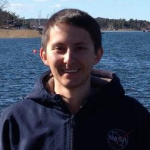
\includegraphics[width=0.15\textwidth]{sam}
\end{wrapfigure} has seven years of experience working as a programmer and communications network engineer. He has been working with microcontrollers and electronics since he was a little boy and will make sure Octanis' brain functions correctly.
\\ \\

\begin{wrapfigure}{l}{0.2\textwidth}
    \centering
    \vspace{-13pt}
    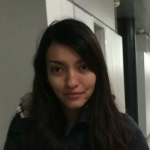
\includegraphics[width=0.15\textwidth]{ana}
\end{wrapfigure}
\paragraph{Ana Roldàn} is a passionate physicist-to-be and involved in every corner of the project. She is not afraid to ask the big questions and inspires everyone with her strong passion for science.
\\ \\

\begin{wrapfigure}{l}{0.2\textwidth}
     \centering
     \vspace{-13pt}
    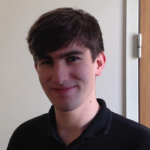
\includegraphics[width=0.15\textwidth]{raf}
\end{wrapfigure} 
\paragraph{Raffael Tschui} is an Electrical Engineer, EPFL, BSc. He has the vital role of energy generation, control and regulation in the project. He keeps the rovers heart beating. He is currently on a mission in Columbia to help an EPFL professor build a bioreactor for water cleaning.
\\ \\

\begin{wrapfigure}{l}{0.2\textwidth}
    \centering
    \vspace{-13pt}
    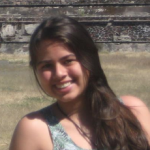
\includegraphics[width=0.15\textwidth]{pam}
\end{wrapfigure} 
\paragraph{Pamela Canjura} has been interested in chemistry since she was five and competes regularly in the Chemistry Olympics. She is working on the chemical analyses that can be done on-board Octanis.
\\ \\


\subsection{Budget}

The following table describes the planned costs with an accuracy of $\pm 20\%$ (m.c. = mission critical): \\ 

\begin{table}[h!]
\centering
\begin{tabular}{ l | c || r }
  Cost Item & Priority & One-Time Costs \\
  \hline
  Rover Solar \& Heating & m.c. & 1000 CHF \\
  Rover Communications & m.c. & 500 CHF \\
  Rover Instruments \& Sensors & m.c. & 500 CHF \\
  Rover Electronics & m.c. & 700 CHF \\
  Rover Mechanics \& Mobility & m.c. & 1000 CHF \\
  Balloon Transportation & opt. & 1500 CHF \\
  \hline \hline
  & & mission critical: 3700 CHF  \\
  & & optional: 1500 CHF \\
\end{tabular}
\caption{General budget.}
\end{table}


The only reoccurring costs are caused by the Iridium Satellite Messenger \cite{iridium}. These range from 0.04-0.12 GBP per message (340 bytes / Message-Out) and a standard line-rental fee of 8 GBP / month. Per-message cost depends on the message volume needed.



\section{Rover Transportation and Deployment}

Octanis 1 is a light-weight rover meaning its total mass will not exceed 2.5kg. Thanks to this there are multiple cost-effective deployment options available which are listed below:

\subsection{Methods of deployment}

\begin{figure}[h!]
	\centering
    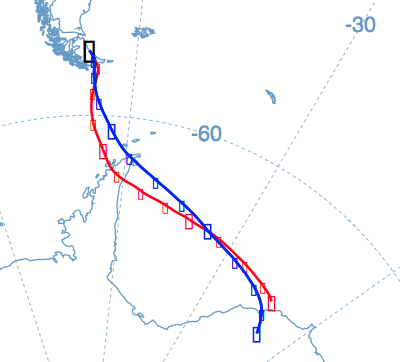
\includegraphics[width=0.4\textwidth]{trajectory}
    \caption{HYSPLIT trajectory simulation starting in Rio Grande, Argentina.}
\end{figure}

\paragraph{High Altitude Balloons} or more commonly known, weather balloons, can be used to bring the rover to its target destination. Helium-filled, they typically float up to an altitude of 30km and a trajectory of hundreds of kilometers can be achieved. However the path of the balloon cannot be controlled and relies on rigorous pre-flight simulations with the HYSPLIT simulation software \cite{hysplit} \cite{hysplitjava}. This is the cheapest method to deploy the rover to Antarctica as it is only required to travel to lower South America, to which commercial flights exist, to launch the rover attached to the balloon. With this benefit comes a higher risk of deployment failure. Even with precise weather models, the weather could suddenly change and move the balloon off its path. That being said, HYSPLIT was already successfully used in numerous ballooning projects like Piccard and Jones' Breitling-Orbiter 3 \cite{hysplitexamples}.
Once the balloon-rover-configuration have reached their target destination, the rover is separated from the balloon and parachutes to the ground. The balloon continues on uncontrolled and will eventually burst or float to the ground after the helium diffuses out.

\begin{figure}[h!]
	\centering
    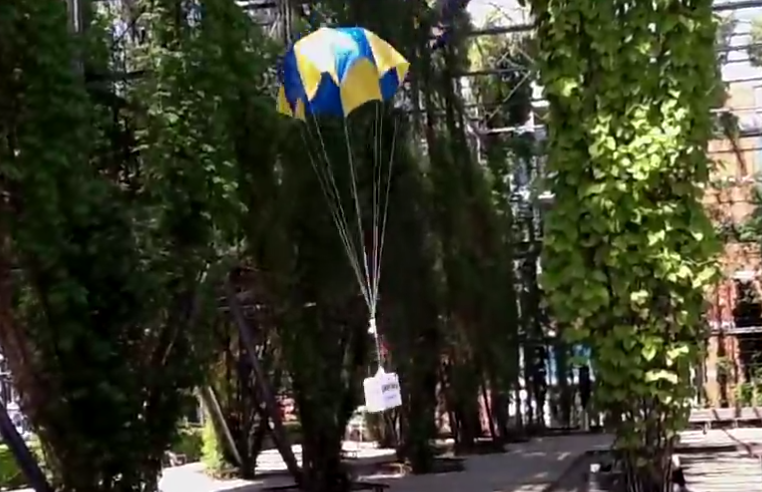
\includegraphics[width=0.5\textwidth]{lowcostchute}
    \caption{Depicted is one of our self-built, low-cost parachutes during a test. }
\end{figure}


\paragraph{Helicopter} - a method to consider is to deploy Octanis out of a helicopter which is already on a specific route. The rover could be given to one of the passengers or attached to the transport cord and detached on demand. Similar to balloon deployment, Octanis would swiftly parachute to the ground and begin its mission.


\paragraph{Manual} deployment is suggested when costs and risk need to be as low as possible. This is by far the easiest method and just means going to the desired location and setting the rover down. Octanis continues on by its own and can return to the set-down location.




\subsection{Environmental Sustainability}
It is desirable to not leave any waste behind as well as it is required by the Antarctic Treaty. Depending on the method of deployment, the total mass and types of materials that will be included on a mission to Antarctica vary. A deployment of the rover to a target out of reach of normal Antarctic expeditions is done by using a High Altitude Balloon or a standard 3kg latex weather balloon. In such a long-distance mission, the rover will be separated from the balloon at the target location and the balloon will continue to fly unattended. Therefore the landing location of the balloon can not be known. Due to the nature of such a long-distance mission, typically the rover is unreachable to any expedition or base - the rover is left for the benefit of information on that location.

In a first step, it is therefore proposed to select a landing site that is in reach of normal Antarctic expeditions or bases. It is even possible to release the rover by other means like bringing it to the location manually or via helicopter.

Concluding, the rover is a construction of various polymers and metals, and a small risk exists that it will end up being uncontrollable due to malfunction. The total rover mass however does not exceed 2.5kg and therefore the pollution produced is small. In the unlikely event of failure, the rover can then be retrieved manually thanks to the last known transmitted location.




\section{Rover Subsystems}

\subsection{Board Computer}
\begin{figure}[h!]
	\centering
    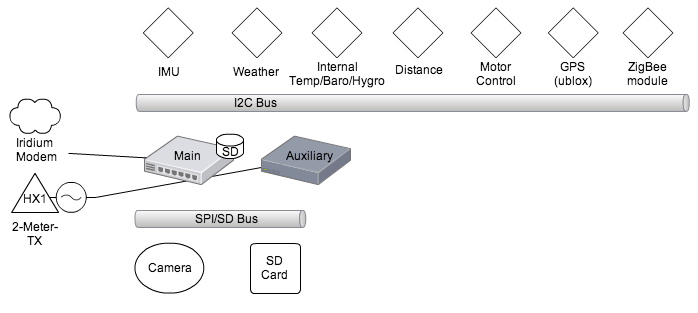
\includegraphics[width=1\textwidth]{schema}
    \caption{Schema of the on-board computing system with peripherals.}
\end{figure} 
The Texas Instruments MSP430 16-bit ultra-low power microcontroller family is the preferred processor choice for the embedded computer system of the rover. The microcontroller will take over most control and regulation tasks, specifically driving, navigation, communications and sensor processing. The system will run a realtime operating system capable of reliably multitasking with prioritised tasks. The computer will interact with the following on-board peripherals:

\begin{itemize}
\item Inertial Measurement Unit: accelerometer, gyroscope, magnetometer, precision barometer.
\item Weather module: temperature, barometer, hygrometer, anemometer.
\item Science instrument: pH probe.
\item Optics module: camera, distance sensors.
\item Drive module: motor controllers, current sensors.
\item Communication: Iridium, APRS, ZigBee.
\item SD card memory.
\item GPS module.
\end{itemize}

An auxiliary computer will take over if the main computer malfunctions. It will try to reset the main computer and if unsuccessful provide basic system functionality.



\subsection{Power}

The energy of the sunlight per square meter is $E_0*sin(\alpha)$ with $E_0=1367 W/m^2$ \cite{solarc} and $\alpha$ the angle between the direct incoming sunrays and the horizontal. For the Antarctic, we can use $\alpha \approx 23.5+90+|\phi|$ where $\phi$ is the latitude, to get an estimate of the maximum energy (i.e. in summer) at a certain geographic point (see fig. 4).


\begin{figure}[h!]
	\centering
    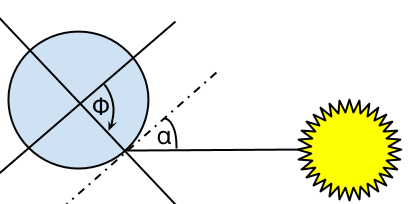
\includegraphics[width=0.6\textwidth]{sun}
    \caption{Octanis rover design concept built after MUSES-CN nanorover.}
\end{figure}


 This would lead to $1050 W/m^2$ for the northmost point of the antarctic (@ 65\degree S) and $545 W/m^2$ at the south pole (@ 90\degree S). Bare in mind that, during the six sunny months this value will oscillate between 0 and the maximum value just calculated \cite{pvedu}. 
Assuming our panels are installed horizontally and considering current solar panel efficiency (around 15-20\%) this means that per square meter we can convert max. 200 W into electrical energy. If we take a pessimistic efficiency and a “radiation mean value” during the 6 months of the mission (just 1/2 of the maximum value) we would need a panel of the size of $0.13m^2$ (@ 65\degree S) to $0.25m^2$ (@ 90\degree S) to output a power of 10 W. But, this didn’t consider the daily oscillation of the radiation angle, nor that it does get night during certain time periods for any point north from the south pole. Therefore, it is more reasonable to take the pessimistic $0.25m^2$ value (also because the energy supply will decrease with bad weather).

To summarise, a panel surface of $0.25m^2$ will provide us with an average (seasonal, daily) power of 10W and these numbers are proportional. 


\subsection{Thermal}

The ultimate priority is to keep the system at -20\degree C or above, which means that all the energy from the solar cell and, if necessary, from the battery will first be used to maintain this goal. The heating system is therefore directly connected between the solar cell and the battery charge controller. It is controlled with electronic comparators that enable one or another energy source to power the heating pads depending on temperature thresholds listed below. The charge controller itself takes care of the temperature limits for charging the battery and switches itself on and off automatically. 


\subsection{Mechanical}
The rover body design (fig. 5) has been substantially influenced by NASA's MUSES-CN nanorover \cite{muses}. The nanorovers design is a unique design as it allows almost complete freedom. We have designed Octanis 1 to be lightweight with a large enough surface area to produce enough solar energy for the mission duration. The body dimensions are roughly 30cm x 30cm x 6cm.

\begin{figure}[h!]
	\centering
    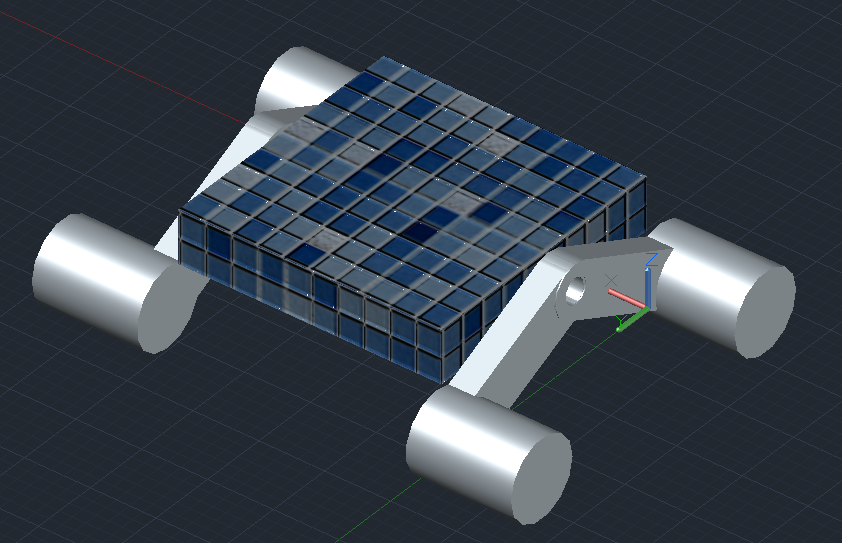
\includegraphics[width=0.5\textwidth]{conceptrover}
    \caption{Octanis rover design concept built after MUSES-CN nanorover.}
\end{figure}

As depicted in figure 6, this rover design allows many orientations for different situations. Main concerns of the mission are energy supply and weather resistance. As the whole rover body is covered with solar cells, the rover can right itself up according to sun position to expose most of its area to sunlight. In harsher weather conditions it is also crucial to make sure snow doesn't cover up the panels. This can be prevented by periodically flipping the rover. Not only snow, but wind can be an issue and sometimes even flipping over the rover. If this occurs, the rover can return to a driving position by actuating the struts. All wheel struts can be rotated around the axis and are fitted with a separate motor each. They are moved through a worm drive to keep them static when they are not rotating without having to apply constant power. \\
Another benefit of this design is it allowing us to build a simpler drilling device. When drilling an ice core, the rover can lower itself to the ground exploiting its own weight as pressure onto the drill. The drill bit just needs to spin and doesn't need to retract into the rover body.

\begin{figure}[h!]
\centering
\begin{tabular}{ c  c  c }
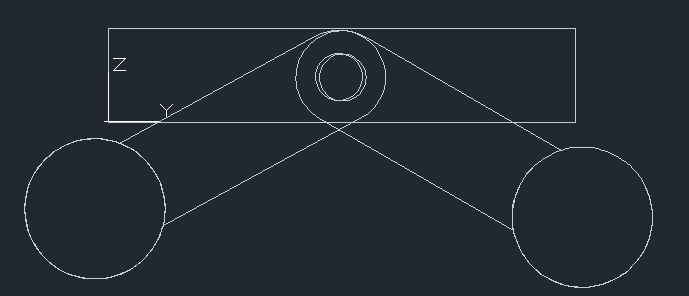
\includegraphics[width=0.3\textwidth]{drive} & 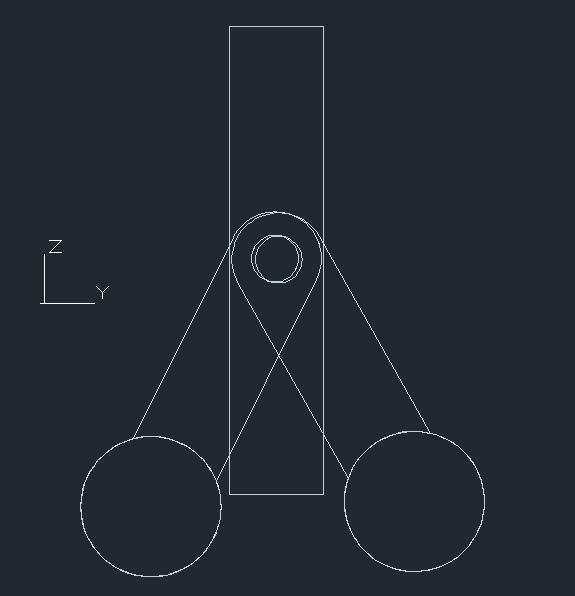
\includegraphics[width=0.25\textwidth]{upright} & 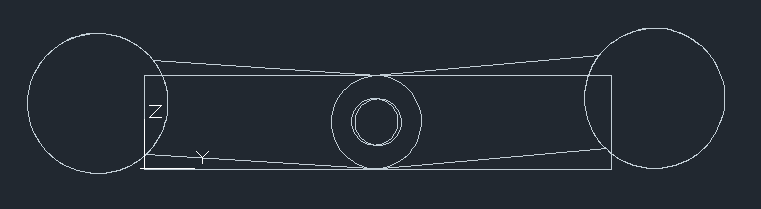
\includegraphics[width=0.4\textwidth]{flat} \\
\end{tabular}
\caption{Different wheel strut configurations l.t.r.: (1) drive mode, (2) solar recharge mode, (3) wind protect mode.}
\end{figure}


\subsection{Mobility}
Snowy and icy terrain will be Octanis' main habitat and so its wheels need to be specifically designed to be wide, lightweight and should provide a good traction going upwards. 
All four wheels will be individually motorised and provide enough torque to move Octanis on an inclination of 30 degrees. Turning can be achieved by rotating the wheels on each side at different speeds. 

\begin{figure}[h!]
	\centering
    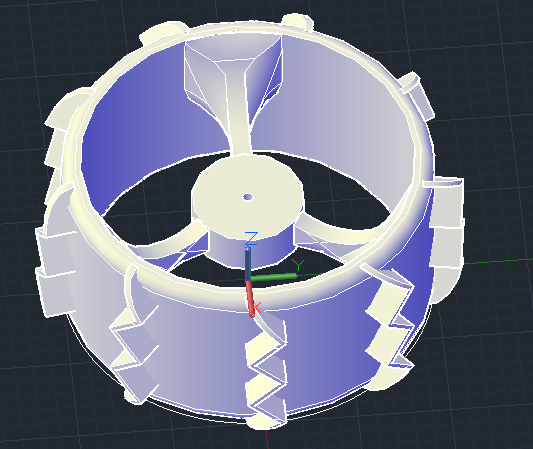
\includegraphics[width=0.4\textwidth]{wheel}
    \caption{Initial wheel design. Fins allow the wheel to dig into the snow while driving providing better traction.}
\end{figure}


An inertial measurement unit (IMU) will be used to know the rovers orientation at any point in time. It consists of a gyroscope, accelerometer, precision barometer and magnetometer. The sensors information is fed back to the control systems that actuate the motors. Should the rover need to go over an obstacle, the wheel struts will be rotated as far as possible so that the rover body is always in a plane parallel to the ground. This minimises the risk of being tipped over and should allow the easy traversal of obstacles higher than the wheel radius and is similar to the rocker-bogie suspension system used on NASAs mars rovers \cite{rockerbogie}. Due to the high risk of overturn caused by wind gusts the passive rocker-bogie design was not chosen, since there would be no simple way of righting back up.

Octanis' top speed is estimated to be at 100cm/min. Disregarding energy availability depending on weather, gives it a daily range of around 1km. There will be two driving modes: discovery and shortest path. \textbf{Discovery mode} will make the rover densely traverse either a preprogrammed circular area of a map or on detecting a certain phenomena (e.g. higher pH levels). \textbf{Shortest path} brings Octanis from waypoint to waypoint using the shortest path. Both methods can be used in combination. Detected obstacles can be stored as landmarks and help build a rough map.

\subsection{Communication}
Regular data transmission is a mission critical feature of the rover. It is achieved by using the Iridium Short Burst Data (SBD) service with the help of the RockBLOCK Iridium 9602 modem \cite{iridium}. This modem allows the transmission of data packets of up to 340 bytes outwards and 270 bytes inwards approximately every 20 seconds. Larger data frames can be fragmented and transmitted with multiple packets. The key to this modem and network is that is available everywhere on Earth at any time, something that cannot be said of the GSM network or even amateur radio. That the modem require just as low power as the GPS on board adds to the list of benefits. Information sent through the Iridium network is automatically sent to a server and uploaded to the project website, where the public can view Octanis' state and data.

Octanis 1 will also be equipped with a 5 watt one-way APRS transmitter, transmitting sensor data and location information on the 2-meter band. This can be received by amateur radio operators (or unlicensed individuals with radio scanners) who are in range. The range of this transmitter is typically hundreds of kilometers when travelling in the sky (i.e. attached to a balloon). On the ground, the range is orders of magnitude smaller.


\subsection{Optical}
Octanis will be able to take snapshots on-demand with a low resolution camera. It is part of an experiment to find out if an image can be efficiently sent via the Iridium network. Additionally we would like to test on-board image processing (e.g. simple feature detection). The optical system is completed by distance sensors that can detect nearest obstacles. It will be evaluated if the Neato XV-11's LIDAR \cite{lidar} can be used or if we should proceed with IR distance sensors.


\subsection{Scientific Instrument}
The preferred scientific instrument for this mission is a ice core drill combined with a pH probe. The drill is able to drill a small 1cm x 5cm ice/snow core, retract it from the cold surface and then melt the sample. The ice/snow-water can be analysed with a pH probe, that is typically a glass electrode, to determine the pH value. Due to the low-cost nature of the sensor to be used, precision cannot be guaranteed by the manufacturer and has to be calibrated and tested by us. It is though assumed that the device will give good readings for comparison of a high quantity of samples.

\pagebreak

\section{Conclusion}
Knowing that this mission is an ambitious one and will have many challenges to be solved on the way, we believe that it is a possible and viable project. When we can achieve our objectives, we will be able to provide the scientific community (including so-called citizen scientists) with a universal and adaptable rover platform. Proving ourselves in the harsh environment of Antarctica means that our rover can survive many other similar environments. \\

We hope to fascinate and inspire students, teachers, artists, entrepreneurs, scientists - in the end all people - for interdisciplinary research, engineering and knowledge sharing, hoping that they will join us on the grand mission to a better world!


\pagebreak
\pagestyle{empty}
\begin{thebibliography}{1}


\bibitem{krishnakant}
  Krishnakant Babanrao Budhavant, Pasumarthi Surya Prakasa Rao, Pramod Digambar Safai,
  \emph{Chemical Composition of Snow-Water and Scavenging Ratios over Costal Antarctica}.
  Aerosol and Air Quality Research, 14: 666–676, 2014.

\bibitem{octanis}
{\em »octanis | discovery and exploration« website} http://octanis.org, 23.6.2014.

\bibitem{iridium}
{\em Rock7 RockBLOCK website} http://rockblock.rock7mobile.com/products-rockblock.php, 25.6.2014.


\bibitem{octanisgithub}
{\em Octanis 1 GitHub repositories website} http://github.com/octanis1, 25.6.2014.

\bibitem{muses}
  Brian H. Wilcox, Ross M. Jones, 
  \emph{The MUSES-CN Nanorover Mission and Related Technology}.
  IEEE Aerospace 2000 Conference, 18.3.1999.


\bibitem{rockerbogie}
  Hayati, S., et. al., 
  \emph{The Rocky 7 Rover: A Mars Sciencecraft Prototype}.
  Proceedings of the 1997 IEEE International Conference on Robotics and Automation, pp. 2458-64, 1997.

\bibitem{hysplit}
  {\em HYSPLIT - Hybrid Single Particle Lagrangian Integrated Trajectory Model }, NOAA, http://www.ready.noaa.gov/HYSPLIT.php, 23.6.2014.

\bibitem{hysplitjava}
  {\em JAVA software to run multiple HYSPLIT simulations to find the optimal parameters for a trajectory}, http://github.com/octanis1/OctanisHYSPLIT, 23.6.2014.

\bibitem{hysplitexamples}
	{\em Ballooning with HYSPLIT}, \\
	http://www.arl.noaa.gov/documents/workshop/Spring2010/Balloon\_flights.ppt, 23.6.2014.

\bibitem{fablab}
	{\em Fab lab definition}, \\
	http://en.wikipedia.org/wiki/Fab\_lab, 25.6.14.

\bibitem{hackerspace}
	{\em Hackerspace definition}, \\
	http://en.wikipedia.org/wiki/Hackerspace, 25.6.14.

\bibitem{pvedu}
	{\em Effect of Light Intensity}, \\
	http://www.pveducation.org/pvcdrom/solar-cell-operation/effect-of-light-intensity, 25.6.14.

\bibitem{lidar}
	{\em Neato XV-11 LIDAR / Piccolo Laser Distance Sensor}, \\
	http://xv11hacking.wikispaces.com/LIDAR+Sensor, 25.6.14.

\bibitem{solarc}
	{\em Solar constant}, \\
	http://en.wikipedia.org/wiki/Solar\_constant, 25.6.14.

\end{thebibliography}

\end{document}